\documentclass[a4paper,11pt]{article}

\usepackage{amsmath}
\usepackage{amssymb}

% for proofs  environment
\usepackage{amsthm}

\usepackage[backend=bibtex]{biblatex}
\bibliography{slides5}

% for probability trees
\usepackage{tikz}
\usetikzlibrary{trees}

% for plots
\usepackage{ pgfplots}
% inserted on suggestion in warning during compilation
\pgfplotsset{compat=1.9}

%for strikethrough text
\usepackage{soul}

%for R source code listing
\usepackage{listings}

%for block quotes
\usepackage{csquotes}

% For not indenting the first line of paragraphs:
\setlength{\parindent}{0pt}
% define the title
\author{John Hancock}
\title{MIT Introduction to Statistics 18.05 Problem Set 2 }
\begin{document}
% generates the title
\maketitle
% insert the table of contents
\tableofcontents
\section{References and License}
We are answering questions in the material from MIT OpenCourseWare
course 18.05, Introduction to Probability and Statistics.

In this document we are answering questions Orloff and Bloom ask in
\cite{slides5}.

Please see the references section for detailed citation information.

The material for the course is licensed under the terms at
\url{http://ocw.mit.edu/terms}.

We use documentation in \cite{latexBarChart} to write \LaTeX source code for this document.
\section{Order variables by size of standard deviation}

In \cite{slides5} Orloff and Bloom give us bar charts of three random variables
and their probability mass functions:

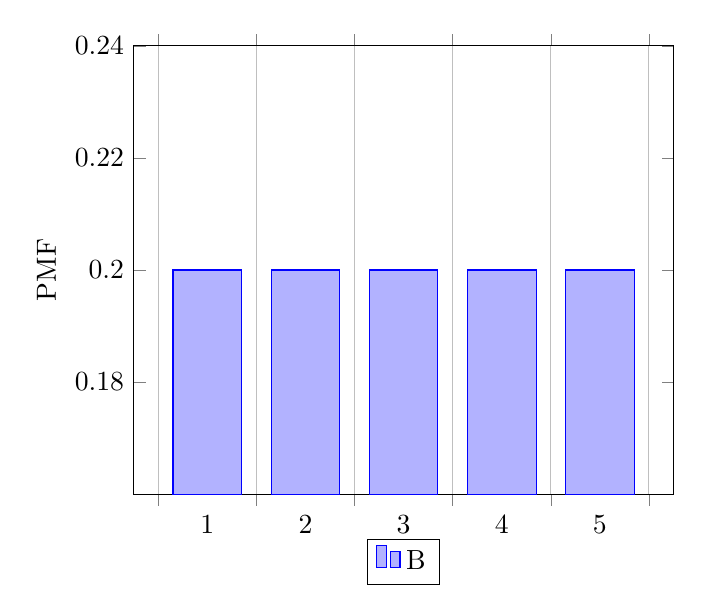
\begin{tikzpicture}
\begin{axis}[
	x tick label style={
		/pgf/number format/1000 sep=},
	ylabel=PMF,
	enlargelimits=0.05,
	legend style={at={(0.5,-0.1)},
	anchor=north,legend columns=-1},
	ybar interval=0.7,
]
\addplot
	coordinates {(1,0.2) (2,0.2)
		 (3,0.2) (4,0.2) (5,0.2) (6, 0.2)};
\legend{B}
\end{axis}
\end{tikzpicture}

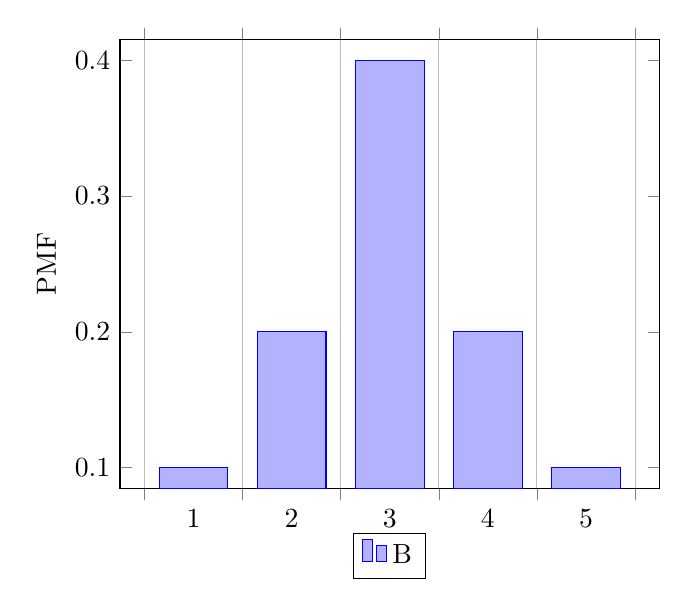
\begin{tikzpicture}
\begin{axis}[
	x tick label style={
		/pgf/number format/1000 sep=},
	ylabel=PMF,
	enlargelimits=0.05,
	legend style={at={(0.5,-0.1)},
	anchor=north,legend columns=-1},
	ybar interval=0.7,
]
\addplot
	coordinates {(1,0.1) (2,0.2)
		 (3,0.4) (4,0.2) (5,0.1) (6, 0.1)};
\legend{B}
\end{axis}
\end{tikzpicture}

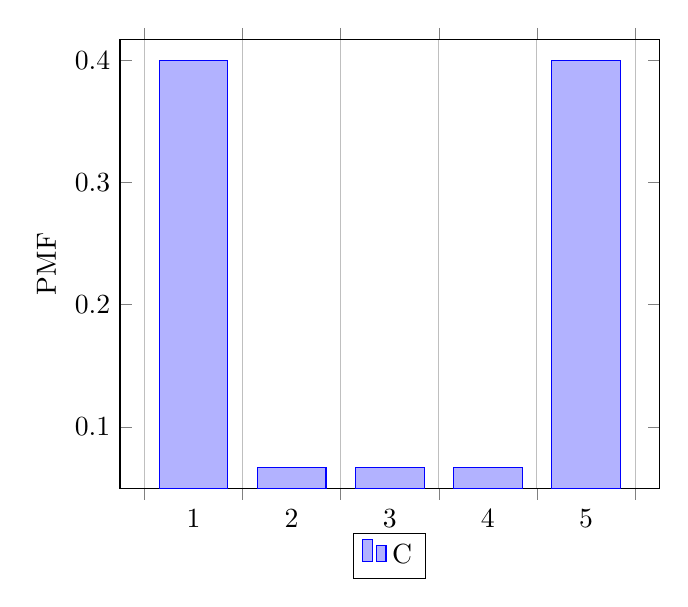
\begin{tikzpicture}
\begin{axis}[
	x tick label style={
		/pgf/number format/1000 sep=},
	ylabel=PMF,
	enlargelimits=0.05,
	legend style={at={(0.5,-0.1)},
	anchor=north,legend columns=-1},
	ybar interval=0.7,
]
\addplot
	coordinates {(1,0.4) (2,0.0667)
		 (3,0.0667) (4,0.0667) (5,0.4) (6,0.4)};
\legend{C}
\end{axis}
\end{tikzpicture}

In \cite{slides5Ans} Orloff and bloom state that the correct order of random
variables by decreasing order of standard deviation is $C$, $A$, $B$.

We disagree with this answer.

The value of $A$ is constant.  Therefore the variance of $A$ is zero.  Hence,
the standard deviation of $A$ is also zero.  Since zero is the minimum value
of a standard deviation, Orloff and Bloom's answer must be incorrect.

We agree that the standard deviation of $C$ is the largest, but $B$ must have
a positive standard deviation greater than zero.  Therefore the order of these
random variables by order of descending standard deviation is $C$, $B$, $A$.

\section{Compute variance and Standard Deviation}

In cite{slides5} Orloff and Bloom ask us to compute the variance and standard
deviation of the following random variable $X$.

\begin{center}
\begin{tabular}{ | c | c | c |  c | c | c | }
  \hline
  values of $X$, $x_{i}$ & 1 & 2 & 3 & 4 & 5  \\ \hline
  PMF $p\left( x_i \right)$ & $\frac{1}{10}$ & $\frac{2}{10}$ & $\frac{4}{10}$
    & $\frac{2}{10}$ & $\frac{1}{10}$ \\ \hline
\end{tabular}
\end{center}

From the table and the definition of expected value, we compute
\begin{equation}
    E\left(X \right) =
      \sum_{i=1}^{n} p\left( x_{i} \right) x_i
\end{equation}

\begin{equation}
      \sum_{i=1}^{n} p\left( x_{i} \right) x_i
  = \frac{1}{10} 1 + \frac{2}{10} 2 + \frac{4}{10} 3 + \frac{2}{10} 4 +
    \frac{1}{10} 5 = \frac{27}{10} = 3.0
\end{equation}

In \cite{reading5a} Orloff and Bloom show that
$\text{Var}\left(X \right) = E \left(X^{2}\right) - E\left( X \right)^{2}$

Substituting the value of $X^{2}$ into the definition of expected value of
a discrete random variable give us:

\begin{equation}
    E\left(X^{2} \right) =
      \sum_{i=1}^{n} p\left( x_{i} \right) x_i^{2}
\end{equation}

And,

\begin{equation}
    \sum_{i=1}^{n} p\left( x_{i} \right) x_i^{2}
    = \frac{1}{10} 1 + \frac{2}{10} 4 + \frac{4}{10} 9 + \frac{2}{10} 16 +
    \frac{1}{10} 25 = \frac{93}{10} = 10.2
\end{equation}

Therefore $\text{Var}\left( X \right) = 10.2 - \left( 3 \right)^{2}
  = 10.2 - 9 = 1.2$.

In \cite{reading5a} Orloff and Bloom give the definition of the standard
deviation of a random variable
$\sigma \left( X \right) = \sqrt{\text{Var}\left(X \right)}$

Therefore the standard deviation of $X$ is $\sqrt{3.05} \approx 1.746 $

\section{Variance of Bernoulli random variable}

The next question Orloff and Bloom ask in the lecture 5 slides is for a proof
that if $X \sim \text{Bernoulli} \left( p \right)$, then
$\text{Var}\left( X \right) = p\left( 1-p \right)$.

Orloff and Bloom prove this in \cite{reading5a}.

\section{Variance of a binomial random variable}

Next, Orloff and Bloom ask for a proof that the variance of a random variable
$X \sim \text{binomial}\left(n, p \right) = np \left( 1 - p \right)$.

Orloff and Bloom also prove this in \cite{reading5a}.

\section{Variance of a sum}

In this section Orloff and Bloom pose the question:

Suppose $X_{1}, X_{2}, \ldots, X_{n}$ are all independent random variables
with $\sigma = 2$.  Define a new random variable, $\bar{X}$ that is the average
of $X_{1}, X_{2}, \ldots, X_{n}$.

They ask, ``What is the standard deviation of $\bar{X}$?''

We know from \cite{reading5a} that, for two independent random variables $X$,
and $Y$, $\text{Var}\left( X + Y \right) = \text{Var}\left( X \right) +
\text{Var}\left( Y \right)$

To extend this property to a sum of more than two independent random variables,
we let $Y=Z+W$, where $Z$, and $W$ are independent random variables.

Then $\text{Var}\left( Z + W \right) = \text{Var}\left( Z \right) +
\text{Var}\left( Z \right)$, and $\text{Var}\left( X + Y\right) =
  \text{Var}\left( X \right) + \text{Var}\left(Z \right)
  + \text{Var}\left(W \right)$.

We continue to rewrite the last term in the sum of variances until we have
an expression on the right hand side of the sum that is the sum of variances
of the independent random variables whose sum we wish to know the variance of.

$\bar{X}$ is the average of the random variables $X_{1}, X_{2}, \ldots, X_{n}$,
so:
\begin{equation}
\bar{X}
  = \frac{1}{n}\sum_{i=1}^{n} X_{i}
\end{equation}

We apply the variance function to both sides of the equation above:


\begin{equation}
\text{Var}\left( \bar{X} \right)
  = \text{Var} \left( \frac{1}{n}\sum_{i=1}^{n} X_{i} \right)
\end{equation}

In \cite{reading5a} Orloff and Bloom show that for constants $a$, $b$:
\begin{equation}
  \text{Var} \left( aX + b \right) = a^{2}\text{Var}\left(X \right)
\end{equation}

Therefore

\begin{equation}
\text{Var}\left( \bar{X} \right)
  = \frac{1}{n^{2}} \text{Var} \left( \sum_{i=1}^{n} X_{i} \right)
\end{equation}

Recall what we showed regarding extending the property of variance to the sum
of multiple independent random variables. Because it is true, we can write

\begin{equation}
\text{Var}\left( \bar{X} \right)
  = \frac{1}{n^{2}} \sum_{i=1}^{n} \text{Var} \left( X_{i} \right)
\end{equation}

Orloff and Bloom give us that $\sigma(X_{i})=2$, so

\begin{equation}
\text{Var}\left( \bar{X} \right)
  = \frac{1}{n^{2}} \sum_{i=1}^{n} \left( 4 \right)
\end{equation}

We evaluate the sum:

\begin{equation}
\text{Var}\left( \bar{X} \right)
  = \frac{1}{n^{2}} 4n
\end{equation}

We simplify the right hand side of the equation above:

\begin{equation}
\text{Var}\left( \bar{X} \right)
  =  \frac{4}{n}
\end{equation}

Since the standard deviation is defined as the square root of the variance, we
apply this definition to arrive at the answer to the question:

\begin{equation}
\sigma \left( \bar{X} \right)
  =  \frac{2}{\sqrt{n}}
\end{equation}

\section{Continuous random variable}
In this section we answer three questions on a continuous random variable $X$
where Orloff and Bloom give us that $X$ has a range $\left[ 0, 2 \right]$, and
the probability density function of $X$ is $f \left( x \right) = cx^{2}$.

subsection{The value of c}
In order to calculate the value of $c$, we use the property of probability
density functions $f\left(x \right)$ Orloff and Bloom give in \cite{reading5b}:

\begin{equation}
  \int_{-\infty}^{\infty} f \left( x \right) dx = 1
\end{equation}

In \cite{reading5b}, Orloff and Bloom give us a note that if we know the range
of the continuous random variable $X$, then in practice we do not integrate
over $\left[ -\infty, \infty \right]$, but over the range of $X$, instead.

Therefore, in the context of what Orloff and Bloom tell us about $X$, and
$f \left(  x \right)$ for this problem:

\begin{equation}
  \int_{0}^{2} f \left( x \right) dx = 1
\end{equation}

Since $f \left( x \right) = cx^{2}$, we know:

\begin{equation}
  \int_{0}^{2}  cx^{2} dx = 1
\end{equation}

The integral of a constant times a function is the constant times the
integral of the function \cite{proofIntProps}.

Therefore:

\begin{equation}
  c \int_{0}^{2}  x^{2} dx = 1
\end{equation}


\printbibliography{}
\end{document}
